\section{Matriz de Confusión}
En el análisis predictivo , una tabla de confusión (a veces también llamado
una matriz de confusión), es una tabla con dos filas y dos columnas que muestra el número
de falsos positivos, falsos negativos, verdaderos positivos y verdaderos negativos. Esto
permite un análisis más detallado que la mera proporción de aciertos (precisión). La
precisión no es una métrica fiable para el rendimiento real de un clasificador, ya que dio
resultados engañosos si el conjunto de datos está desequilibrado (es decir, cuando el
número de muestras en diferentes clases varían en gran medida). Por ejemplo, si había 95
gatos y sólo 5 perros en el conjunto de datos, el clasificador podría fácilmente estar
sesgada en la clasificación de todas las muestras como los gatos. La precisión global sería 95\%, pero en la práctica el clasificador tendría una tasa de reconocimiento 100\% para la
clase de gato, pero una tasa de reconocimiento 0\% para la clase de perro \cite{30Mconfusion}.

Suponiendo que la matriz de confusión anterior, su correspondiente tabla de
confusión, para la clase de gato, sería la siguiente:

\begin{table}[!htb]
    \centering
    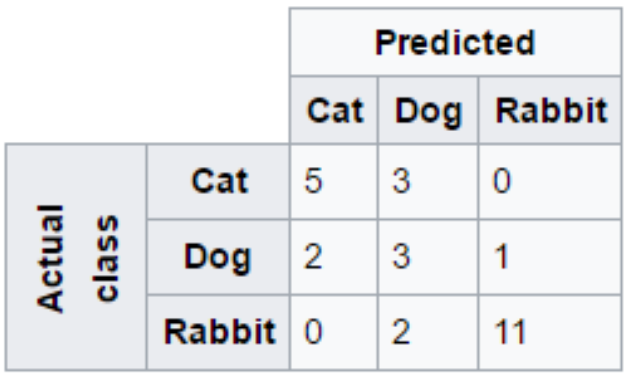
\includegraphics[width=50mm]{Imagenes/matriz_confusion.png}
    \caption{Ejemplo de una matriz de confusión}
    \label{tab:matriz_confusion}
   \vspace{0.5cm}
    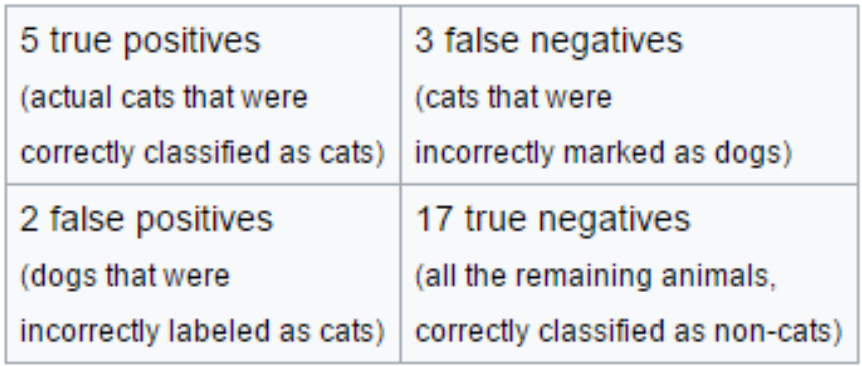
\includegraphics[width=50mm]{Imagenes/interpretacion_matriz_confusion.png}
    \caption{Interpretación de la matriz de confusión}
    \label{tab:inter_matriz_confusion}
    
\end{table}




\section{Machine Learning}
A grandes rasgos se puede decir que el Machine Learning o aprendizaje
automático es un tipo de Inteligencia Artificial dirigido al desarrollo de técnicas para que
las máquinas puedan aprender y tomar decisiones por sí mismas.
Este aprendizaje es posible gracias a la detección de patrones dentro de un
conjunto de datos de manera que es el propio programa el que predice qué situaciones
podrían darse o no. Estos cálculos son los que les permiten aprender para, finalmente,
generar decisiones y resultados fiables \cite{31MLApplications}.

\section{Aplicaciones de Machine Learning}
El aprendizaje automático cuenta con tantas aplicaciones como imaginemos,
pudiéndose adaptar a tantas situaciones como datos con los que contemos. Motores de
búsqueda, diagnósticos médicos, reconocimiento del habla y del lenguaje, robótica, entre
otras, éstas son algunas de las actividades de nuestro día a día que se ven impulsadas por
el \textit{machine learning} \cite{31MLApplications}:


\begin{itemize}
\item Detección de rostro. Podemos verlo en nuestras cámaras móviles.
\item Reconocimiento facial, de voz o de objetos.
\item 	Buscadores. Para mejorar los resultados y sugerencias de búsqueda.
\item Anti-spam. Mediante el uso de etiquetas.
\item Anti-virus. Para la detección de software malicioso.
\item Genética. Por ejemplo, en la clasificación de secuencias de ADN.

\item Predicción y pronósticos del clima, tráfico o para evitar fallos tecnológicos en
equipos.

\item Comprensión de textos. Se aplica a resúmenes estructurados de noticias o
comentarios sobre un tema específico.

\item Vehículos autónomos y robots.

\item Métodos de optimización más rápidos y flexibles. Se evalúa qué momento es el
adecuado para una tarea concreta.

\item Análisis de imágenes de alta calidad.

\item Análisis de datos económicos para operar en el mercado de valores o evitar el
fraude en transacciones.

\item Análisis de comportamiento de consumo y productividad. Para la identificación
de clientes potenciales, prever qué empleados pueden ser más rentables, adaptar
servicios a las necesidades del usuario y otros

\end{itemize}


\section{Early Stopping}

Durante el entrenamiento de redes neuronales, numerosas decisiones tienen que
ser tomadas con respecto a los ajustes (hiperparámetro) utilizados, con el fin de obtener
un buen rendimiento. Tales hiperparámetro son el número de epoch de formación: es
decir, el número de veces que utilizaremos el conjunto de datos. Si utilizamos muy pocas
épocas, podríamos ocasionar \textit{underfit} (es decir, no aprende todo lo que podamos de los
datos de entrenamiento); si usamos demasiadas epoch, podríamos ocasionar un \textit{overfit} (es decir, colocar el "ruido" en los datos de entrenamiento, y no la señal).

Early Stopping intenta eliminar la necesidad de configurar manualmente este
valor. También se puede considerar un tipo de método de regularización (como L1 / L2
y el dropout) en que se puede detener la red de \textit{overfitting}. 

La idea detrás de Early Stopping es relativamente simple \cite{32Stopping}:


\begin{itemize}
 \item Los datos están divididos en training y test.
 \item Al final de cada epoch (o, cada N epoch):
  \begin{itemize}
  \item Evaluar el rendimiento de la red en el equipo de prueba
  \item Si la red supera al mejor modelo anterior: guardar una copia de la red en
  la epoch actual
  \end{itemize}
  \item Tomar como modelo final el modelo que tiene el mejor rendimiento del test
  Esto se muestra gráficamente a continuación
\end{itemize}


\begin{figure}[!htb]
    \centering
    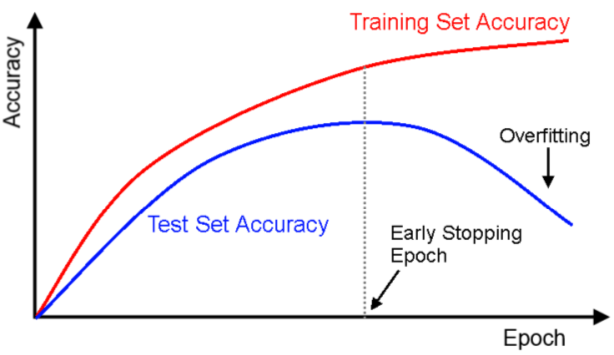
\includegraphics[width=100mm]{Imagenes/early_stopping.png}
    \caption{Representación gráfica deEarly Stopping}
    \label{fig:early_stopping}
    
\end{figure}


